% 中山大学科技类及IT类实验报告文档类(LaTeX模板)
\documentclass{sysucseexp}
\usepackage{fontspec,inconsolata,url}
\setmainfont{Times New Roman}
\setmonofont{Consolas}

% 载入需要的宏包
\input{settings/packages.tex}
% 进行必要的设置
\input{settings/format.tex}
% 专用术语宏命令进行必要的设置
\input{settings/terms.tex}

% 设置封面基本信息，\linebreak 前面不要有空格，
% 中文之间的空格无法消除
% 另，在\sysucseset中不可以出现空行
\sysucseset{
  college = {计算机学院},            % 学院名称
  projname = {计算复杂性理论实验},       % 实践课程名称
  title = {近似算法实现实验报告},    % 实验报告题目
  stunoleader = {23336150},              % 组长学号
  authorleader = {刘昊},             % 组长姓名
  stunoone = {23336203},              % 组员1学号
  authorone = {任意嵘},             % 组员1姓名
  stunotwo = {23336193},              % 组员2学号
  authortwo = {彭怡萱},             % 组员2姓名
  major = {计算机科学与技术},          % 专业
  adviser = {冯剑琳},                   % 指导教师姓名
  startdate = {2026年6月11日},        % 实验起始日期
  enddate = {6月23日}        % 实验结束日期
}

\begin{document} %在document环境中撰写文档

%%%%%%%%%%%%%%%%%%%%%%%%%%%%%%%%%%%%%%%%
% 封面及目录，无需改动此处代码
\makecover
% 目录
\tableofcontents
\cleardoublepage
% 设置正文页眉页脚格式，并重新设置页码为1
\pagestyle{main} % 无页眉，页码在页脚居中
%%%%%%%%%%%%%%%%%%%%%%%%%%%%%%%%%%%%%%%%

% 排版正文内容
\section{实验内容}

本次实验实现两个经典近似算法，并对算法输出、运行时间和近似效果进行记录与分析。

\subsection{任务一：MAX-3SAT 随机近似算法}

MAX-3SAT 的输入是由若干 3-文字子句组成的布尔公式。设公式共有 $m$ 个子句，实验目标是寻找一组变量赋值，使满足的子句数量至少达到
\[
  \left\lceil \frac{7m}{8} \right\rceil .
\]
对于任意一个恰含 3 个不同变量且不同时包含同一变量及其否定的子句，均匀随机赋值使其不满足的概率为 $1/8$，满足概率为 $7/8$。因此随机赋值满足的期望子句数为 $7m/8$。程序实现了反复随机生成赋值、统计满足子句数、达到阈值后停止的 Las Vegas 风格随机算法。

在本优化版本中，为提升实际满足子句数并避免极端情况下长时间循环，求解器额外提供了两个工程化选项：一是 \path{max_attempts} 最大随机尝试次数，二是 \path{use_hill_climb} 局部爬山改进。关闭局部爬山时，算法退化为规格说明中的纯随机重复算法；实验默认开启局部爬山，以观察满足子句数和运行时间的变化。

\subsection{任务二：METRIC-TSP 二近似算法}

METRIC-TSP 的输入为满足三角不等式的带权完全图。本实验按规格从二维城市坐标读取实例，使用
\[
  c(u,v)=\left\lceil \sqrt{(x_u-x_v)^2+(y_u-y_v)^2} \right\rceil
\]
构造边权，从而得到满足三角不等式的完全图。

近似算法采用 MST+DFS 的二近似框架：先计算最小生成树，任选一个根节点做 DFS 遍历，再按首次访问顺序构造回路。由于任意 Hamilton 回路删去一条边后是一棵生成树，有 $\mathrm{cost(MST)}\leq \mathrm{OPT}$；又因为 DFS 所对应的树边往返总代价不超过 $2\mathrm{cost(MST)}$，并且在满足三角不等式时跳过重复顶点不会增加总代价，所以最终近似回路满足
\[
  \mathrm{cost(tour)} \leq 2\mathrm{OPT}.
\]
为计算近似比例，程序还对小规模测试用例用回溯剪枝求出精确最优 TSP 回路。

\subsection{运行方式}

项目根目录下执行如下命令即可运行所有测试用例：

{\small
\begin{verbatim}
python src/main.py --all
\end{verbatim}
}

MAX-3SAT 的规模实验可以执行：

{\small
\begin{verbatim}
python run_max3sat_scaling_experiment.py
\end{verbatim}
}

\section{模块设计思路}

\subsection{项目结构}

项目按问题类型拆分为两个子模块，并将输入、输出与工具代码分离：

\begin{itemize}
  \item \path{src/max3sat/models.py}：定义文字、子句和公式，负责子句求值、满足子句统计以及 $7/8$ 阈值计算。
  \item \path{src/max3sat/parser.py}：解析固定公式输入，解析随机生成配置，并按种子生成可复现实例。
  \item \path{src/max3sat/solver.py}：实现随机赋值算法和可选局部爬山优化，记录随机赋值次数、子句检查次数、翻转次数和运行时间。
  \item \path{src/metric_tsp/models.py}：定义城市、边和带权完全图，按向上取整欧氏距离生成边权。
  \item \path{src/metric_tsp/mst.py}：使用 Kruskal 算法和并查集计算 MST。
  \item \path{src/metric_tsp/dfs.py}：将 MST 转为邻接表并执行 DFS，按访问顺序构造近似 TSP 回路。
  \item \path{src/metric_tsp/solver.py}：组织 TSP 近似求解流程，并用回溯剪枝计算最优解用于比较。
  \item \path{src/main.py}：命令行入口，负责根据任务参数调用相应模块并把结果写入 \path{output/}。
\end{itemize}

\subsection{MAX-3SAT 模块设计}

MAX-3SAT 的核心数据结构是 \path{Formula}。公式对象维护子句列表和变量集合，\path{threshold} 属性直接返回 $\lceil 7m/8\rceil$，从而保证求解器不需要重复处理阈值逻辑。解析器逐行读取输入文件，每行必须恰好包含 3 个文字，并检查同一子句中变量不重复、不得同时出现变量及其否定。

随机生成器使用 \path{random.Random(seed)} 建立局部随机数生成器；在每个子句中先从 $n$ 个变量中无放回抽取 3 个变量，再独立决定每个文字是否取否定。这样相同的 \path{seed}、变量数和子句数会得到相同公式，满足实验可复现要求。

求解器以随机赋值为主流程。每产生一组赋值就统计一次满足子句数；如果未达到阈值且启用局部爬山，就随机打乱变量顺序，尝试翻转单个变量，只接受能提高满足子句数的翻转。该策略不改变阈值判定标准，但可以在较大随机实例上明显提高最终满足子句数量。

\subsection{METRIC-TSP 模块设计}

METRIC-TSP 先由城市坐标构造完全图。程序对每对不同城市计算向上取整的欧氏距离，并同时写入边列表、邻接表和权重查询表；后续 MST、DFS、回路代价计算都基于同一个 \path{WeightedGraph} 对象，避免重复计算边权。

MST 采用 Kruskal 算法：按边权、端点名称排序所有边，用并查集维护连通分量，每次选择不会成环的最小边，直到选出 $|V|-1$ 条边。DFS 模块先根据 MST 边集建立无向邻接表，并对邻居排序以保证输出顺序稳定。近似回路直接由 DFS 首次访问顺序加回起点构成。

最优 TSP 回路只用于小规模实例的近似比例评估。相比直接枚举全排列，程序使用回溯逐步构造路径，当当前路径代价已经不小于已知最优解时立即剪枝，减少无效搜索。

\section{关键代码展示}

\subsection{MAX-3SAT 阈值与公式求值}

\path{Formula} 将阈值计算和满足子句统计封装在模型层，求解器只需调用统一接口。

{\small
\begin{verbatim}
@property
def threshold(self) -> int:
    return math.ceil(7 / 8 * self.num_clauses)

def count_satisfied(self, assignment: Dict[str, bool]) -> int:
    return sum(1 for clause in self.clauses
               if clause.is_satisfied(assignment))
\end{verbatim}
}

\subsection{MAX-3SAT 随机求解流程}

求解器每轮生成一组随机赋值，统计满足子句数，并在达到 $\lceil 7m/8\rceil$ 后停止。实验版本同时记录随机赋值次数、子句检查次数和运行时间。

{\small
\begin{verbatim}
while random_assignments < max_attempts:
    random_assignments += 1
    assignment = random_assignment(variables, rng)
    satisfied_count, checks = count_satisfied_with_checks(assignment)
    clause_checks += checks

    if use_hill_climb and satisfied_count < threshold:
        assignment, satisfied_count, flips, hc_checks = \
            hill_climb_improve(formula, assignment, rng, max_steps=100)
        hill_flips += flips
        clause_checks += hc_checks

    if satisfied_count >= threshold:
        break
\end{verbatim}
}

局部爬山部分只接受能提升当前满足子句数的变量翻转；若一轮变量扫描没有提升，则停止局部搜索。

{\small
\begin{verbatim}
for v in vars_shuffled:
    flips += 1
    current[v] = not current[v]
    new_score, local_checks = count_satisfied_local(current)
    checks += local_checks
    if new_score > current_score:
        current_score = new_score
        improved = True
        break
    current[v] = not current[v]
\end{verbatim}
}

\subsection{Kruskal 最小生成树}

Kruskal 算法先按权重排序所有边，再用并查集判断加入边后是否成环。该实现没有调用第三方图算法库。

{\small
\begin{verbatim}
def kruskal(graph: WeightedGraph) -> List[Edge]:
    city_to_idx = {name: i for i, name in enumerate(graph.city_names)}
    sorted_edges = sorted(graph.edges, key=lambda e: (e.weight, e.u, e.v))
    uf = UnionFind(graph.num_cities)
    mst_edges: List[Edge] = []

    for edge in sorted_edges:
        u_idx = city_to_idx[edge.u]
        v_idx = city_to_idx[edge.v]
        if uf.union(u_idx, v_idx):
            mst_edges.append(edge)
            if len(mst_edges) == graph.num_cities - 1:
                break
    return mst_edges
\end{verbatim}
}

\subsection{METRIC-TSP 近似流程与精确解剪枝}

近似流程严格对应“构造 MST、DFS、回路、计算代价”的步骤；随后用剪枝回溯计算最优解，以输出近似比例。

{\small
\begin{verbatim}
mst_edges = kruskal(graph)
mst_cost = mst_total_cost(mst_edges)
dfs_order = dfs_traversal(mst_edges, root)
tsp_tour = build_tsp_tour(dfs_order)
tsp_cost = compute_tour_cost(tsp_tour, graph)

optimal_tour, optimal_cost = brute_force_optimal_with_pruning(graph)
approximation_ratio = tsp_cost / optimal_cost
\end{verbatim}
}

回溯剪枝的关键是：若当前部分路径代价已经不优于已知最优解，则无需继续扩展。

{\small
\begin{verbatim}
def backtrack(path: List[str], used: set, current_cost: int):
    nonlocal best_cost, best_tour
    if current_cost >= best_cost:
        return
    if len(path) == n:
        tour = path + [start]
        total_cost = current_cost + graph.get_weight(path[-1], start)
        if total_cost < best_cost:
            best_cost = total_cost
            best_tour = tour
        return
\end{verbatim}
}

\section{运行结果展示}

\subsection{MAX-3SAT 固定测试用例}

固定测试用例包含 6 个变量和 6 个子句，目标阈值为 $\lceil 7\times 6/8\rceil=6$。程序一次随机赋值即得到满足全部子句的解。

\begin{table}[htbp]
  \centering
  \caption{MAX-3SAT 固定测试用例结果}
  \begin{tabular}{cccccc}
    \toprule
    变量数 & 子句数 & 阈值 & 满足子句数 & 随机赋值次数 & 运行时间 \\
    \midrule
    6 & 6 & 6 & 6/6 & 1 & 0.0004s \\
    \bottomrule
  \end{tabular}
\end{table}

输出赋值为 $x_1,\ldots,x_6$ 全部取 \path{True}，满足子句编号为 C1--C6，说明固定测试用例满足实验输出要求。

\subsection{MAX-3SAT 随机规模实验}

规模实验固定随机种子为 2026，子句数取变量数的 4 倍。表中平均值来自 \path{output/max3sat/max3sat_scaling_summary.txt}；由于当前每个规模只运行一个种子，平均值等于该次运行结果。

\begin{table}[htbp]
  \centering
  \caption{MAX-3SAT 随机生成测试结果}
  \begin{tabular}{cccccccc}
    \toprule
    变量数 & 子句数 & 阈值 & 满足子句数 & 随机赋值 & 子句检查 & 爬山翻转 & 时间 \\
    \midrule
    50  & 200  & 175 & 192/200  & 1.00 & 32000   & 159  & 0.0343s \\
    100 & 400  & 350 & 352/400  & 1.00 & 400     & 0    & 0.0004s \\
    150 & 600  & 525 & 585/600  & 1.00 & 498600  & 830  & 0.4743s \\
    200 & 800  & 700 & 781/800  & 1.00 & 955200  & 1193 & 0.8984s \\
    250 & 1000 & 875 & 979/1000 & 1.00 & 1152000 & 1151 & 1.1224s \\
    \bottomrule
  \end{tabular}
\end{table}

\begin{figure}[htbp]
  \centering
  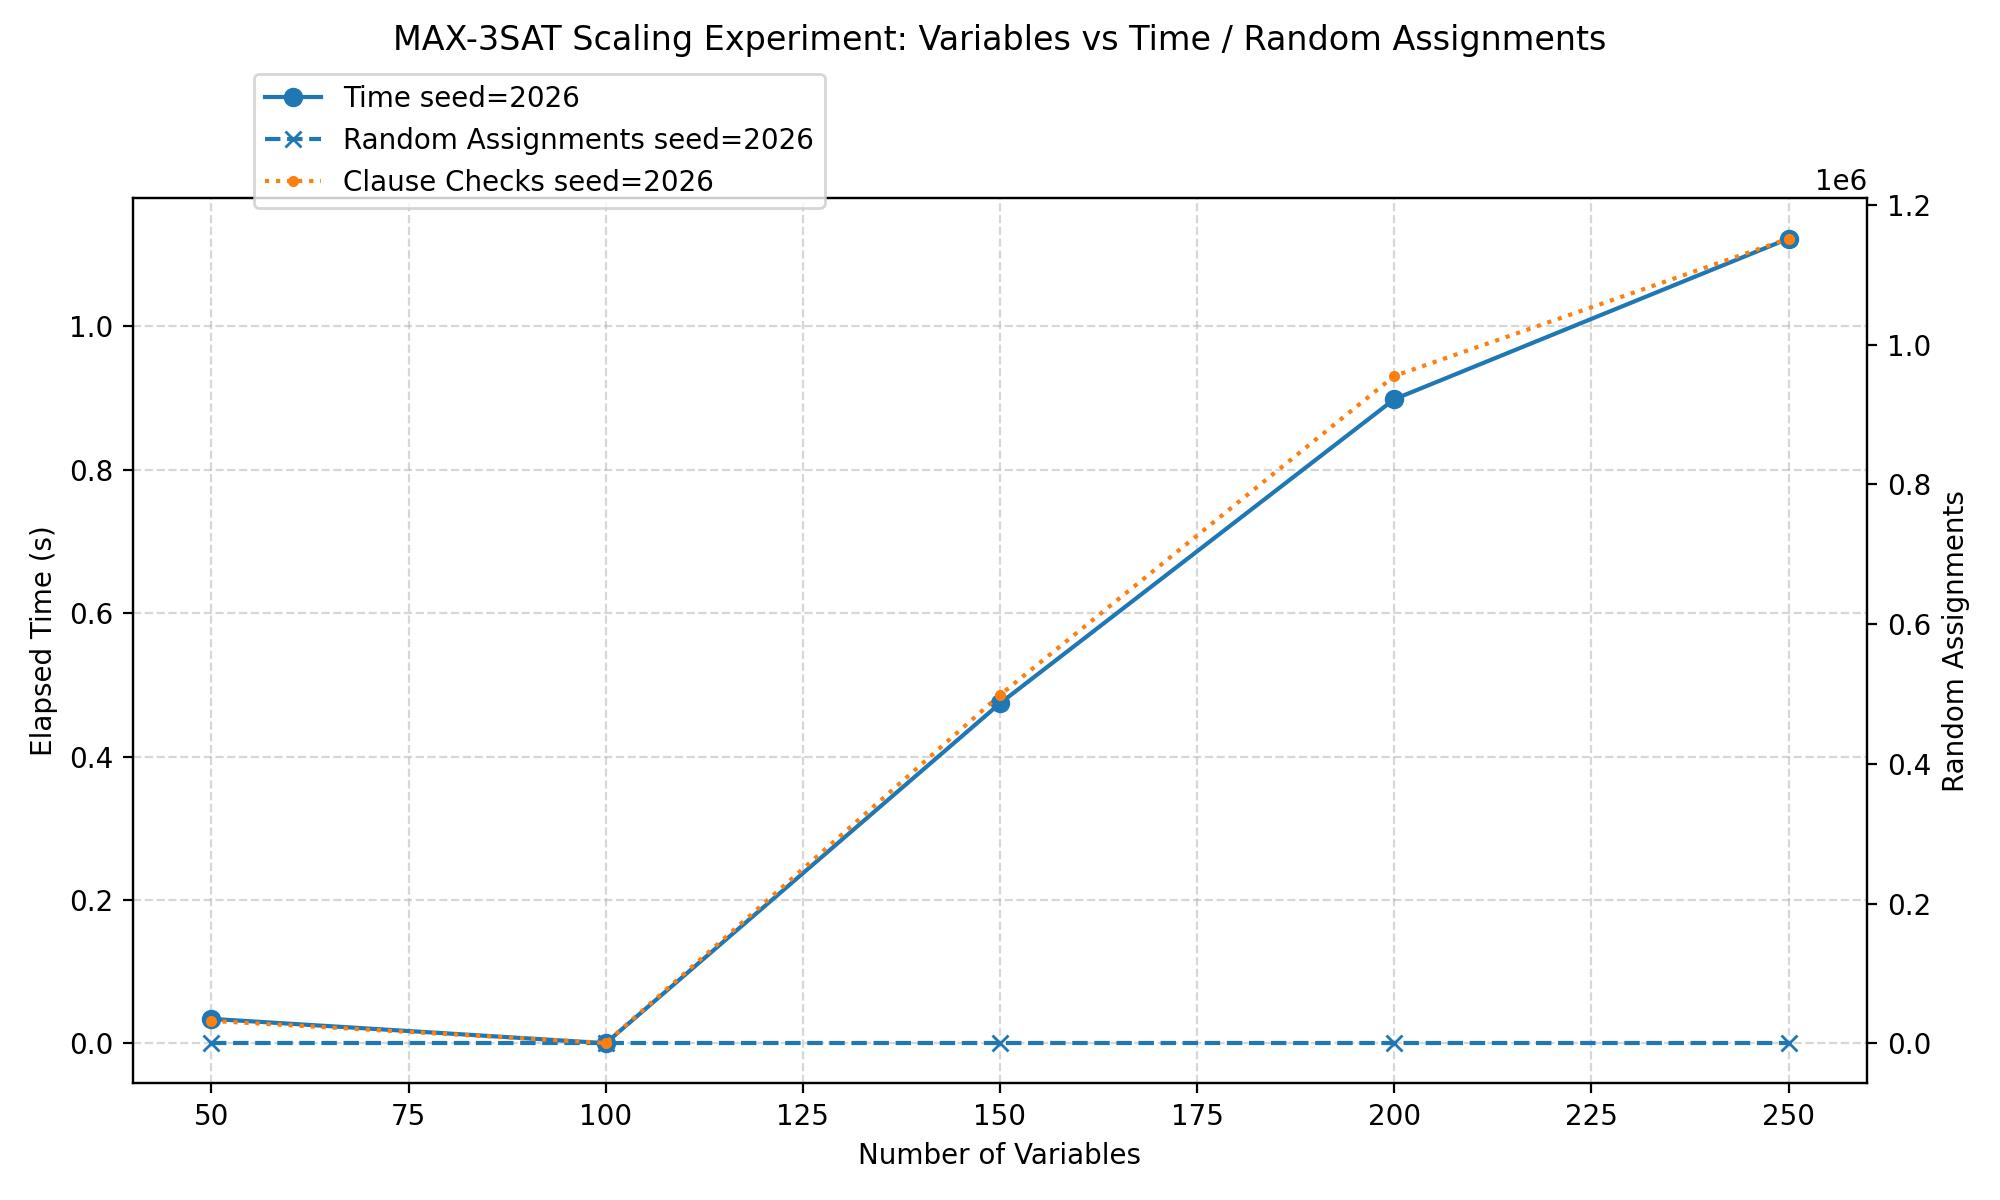
\includegraphics[width=0.88\textwidth]{figs/max3sat-scaling-plot.png}
  \caption{MAX-3SAT 规模实验曲线}
\end{figure}

从结果看，所有随机实例都达到 $\lceil 7m/8\rceil$ 阈值，成功率为 1.00。随机赋值次数均为 1，说明这些随机实例中第一组赋值或其局部改进已经足以达到理论阈值。运行时间主要受局部爬山中的重复子句评估影响：当初始随机赋值已经达到阈值时，例如 $n=100,m=400$，无需爬山，运行时间只有 0.0004s；当需要较多翻转尝试时，子句检查次数上升到几十万至百万级，运行时间也随之增加到约 0.47s--1.12s。该现象说明局部爬山能提高满足子句数量，但代价是更多子句评估开销。

\subsection{METRIC-TSP 测试用例}

任务二共测试两个 6 城市实例。两个实例均从坐标构造满足三角不等式的完全图，并输出 MST、DFS 顺序、近似回路、最优回路和近似比例。

\begin{table}[htbp]
  \centering
  \caption{METRIC-TSP 测试结果}
  \begin{tabular}{ccccccc}
    \toprule
    用例 & 根节点 & MST 代价 & 近似回路代价 & $2\times$MST & 最优代价 & 近似比例 \\
    \midrule
    sample & a & 6 & 10 & 12 & 8  & 1.250 \\
    extra  & s & 8 & 12 & 16 & 10 & 1.200 \\
    \bottomrule
  \end{tabular}
\end{table}

样例 \path{sample.txt} 的 MST 边集为 $(a,b,1)$、$(a,d,1)$、$(b,c,1)$、$(b,e,1)$、$(c,f,2)$，DFS 顺序为
\[
  a \rightarrow b \rightarrow c \rightarrow f \rightarrow e \rightarrow d .
\]
构造得到近似回路
\[
  a \rightarrow b \rightarrow c \rightarrow f \rightarrow e \rightarrow d \rightarrow a,
\]
总代价为 10；最优回路代价为 8，近似比例为 $10/8=1.250$。

额外用例 \path{extra_case.txt} 的 DFS 顺序为
\[
  s \rightarrow a \rightarrow b \rightarrow c \rightarrow d \rightarrow e,
\]
近似回路总代价为 12；最优回路代价为 10，近似比例为 $12/10=1.200$。

两个测试用例中均有 $\mathrm{cost(tour)}\leq 2\times\mathrm{cost(MST)}$，且近似比例都小于 2，符合 METRIC-TSP 二近似算法的理论保证。由于实例规模为 6 个城市，回溯剪枝求最优回路耗时很小，输出文件中运行时间均显示为 0.000s 量级。

\end{document}
